\documentclass[1p]{elsarticle_modified}
%\bibliographystyle{elsarticle-num}

%\usepackage[colorlinks]{hyperref}
%\usepackage{abbrmath_seonhwa} %\Abb, \Ascr, \Acal ,\Abf, \Afrak
\usepackage{amsfonts}
\usepackage{amssymb}
\usepackage{amsmath}
\usepackage{amsthm}
\usepackage{scalefnt}
\usepackage{amsbsy}
\usepackage{kotex}
\usepackage{caption}
\usepackage{subfig}
\usepackage{color}
\usepackage{graphicx}
\usepackage{xcolor} %% white, black, red, green, blue, cyan, magenta, yellow
\usepackage{float}
\usepackage{setspace}
\usepackage{hyperref}

\usepackage{tikz}
\usetikzlibrary{arrows}

\usepackage{multirow}
\usepackage{array} % fixed length table
\usepackage{hhline}

%%%%%%%%%%%%%%%%%%%%%
\makeatletter
\renewcommand*\env@matrix[1][\arraystretch]{%
	\edef\arraystretch{#1}%
	\hskip -\arraycolsep
	\let\@ifnextchar\new@ifnextchar
	\array{*\c@MaxMatrixCols c}}
\makeatother %https://tex.stackexchange.com/questions/14071/how-can-i-increase-the-line-spacing-in-a-matrix
%%%%%%%%%%%%%%%

\usepackage[normalem]{ulem}

\newcommand{\msout}[1]{\ifmmode\text{\sout{\ensuremath{#1}}}\else\sout{#1}\fi}
%SOURCE: \msout is \stkout macro in https://tex.stackexchange.com/questions/20609/strikeout-in-math-mode

\newcommand{\cancel}[1]{
	\ifmmode
	{\color{red}\msout{#1}}
	\else
	{\color{red}\sout{#1}}
	\fi
}

\newcommand{\add}[1]{
	{\color{blue}\uwave{#1}}
}

\newcommand{\replace}[2]{
	\ifmmode
	{\color{red}\msout{#1}}{\color{blue}\uwave{#2}}
	\else
	{\color{red}\sout{#1}}{\color{blue}\uwave{#2}}
	\fi
}

\newcommand{\Sol}{\mathcal{S}} %segment
\newcommand{\D}{D} %diagram
\newcommand{\A}{\mathcal{A}} %arc


%%%%%%%%%%%%%%%%%%%%%%%%%%%%%5 test

\def\sl{\operatorname{\textup{SL}}(2,\Cbb)}
\def\psl{\operatorname{\textup{PSL}}(2,\Cbb)}
\def\quan{\mkern 1mu \triangleright \mkern 1mu}

\theoremstyle{definition}
\newtheorem{thm}{Theorem}[section]
\newtheorem{prop}[thm]{Proposition}
\newtheorem{lem}[thm]{Lemma}
\newtheorem{ques}[thm]{Question}
\newtheorem{cor}[thm]{Corollary}
\newtheorem{defn}[thm]{Definition}
\newtheorem{exam}[thm]{Example}
\newtheorem{rmk}[thm]{Remark}
\newtheorem{alg}[thm]{Algorithm}

\newcommand{\I}{\sqrt{-1}}
\begin{document}

%\begin{frontmatter}
%
%\title{Boundary parabolic representations of knots up to 8 crossings}
%
%%% Group authors per affiliation:
%\author{Yunhi Cho} 
%\address{Department of Mathematics, University of Seoul, Seoul, Korea}
%\ead{yhcho@uos.ac.kr}
%
%
%\author{Seonhwa Kim} %\fnref{s_kim}}
%\address{Center for Geometry and Physics, Institute for Basic Science, Pohang, 37673, Korea}
%\ead{ryeona17@ibs.re.kr}
%
%\author{Hyuk Kim}
%\address{Department of Mathematical Sciences, Seoul National University, Seoul 08826, Korea}
%\ead{hyukkim@snu.ac.kr}
%
%\author{Seokbeom Yoon}
%\address{Department of Mathematical Sciences, Seoul National University, Seoul, 08826,  Korea}
%\ead{sbyoon15@snu.ac.kr}
%
%\begin{abstract}
%We find all boundary parabolic representation of knots up to 8 crossings.
%
%\end{abstract}
%\begin{keyword}
%    \MSC[2010] 57M25 
%\end{keyword}
%
%\end{frontmatter}

%\linenumbers
%\tableofcontents
%
\newcommand\colored[1]{\textcolor{white}{\rule[-0.35ex]{0.8em}{1.4ex}}\kern-0.8em\color{red} #1}%
%\newcommand\colored[1]{\textcolor{white}{ #1}\kern-2.17ex	\textcolor{white}{ #1}\kern-1.81ex	\textcolor{white}{ #1}\kern-2.15ex\color{red}#1	}

{\Large $\underline{11a_{93}~(K11a_{93})}$}

\setlength{\tabcolsep}{10pt}
\renewcommand{\arraystretch}{1.6}
\vspace{1cm}\begin{tabular}{m{100pt}>{\centering\arraybackslash}m{274pt}}
\multirow{5}{120pt}{
	\centering
	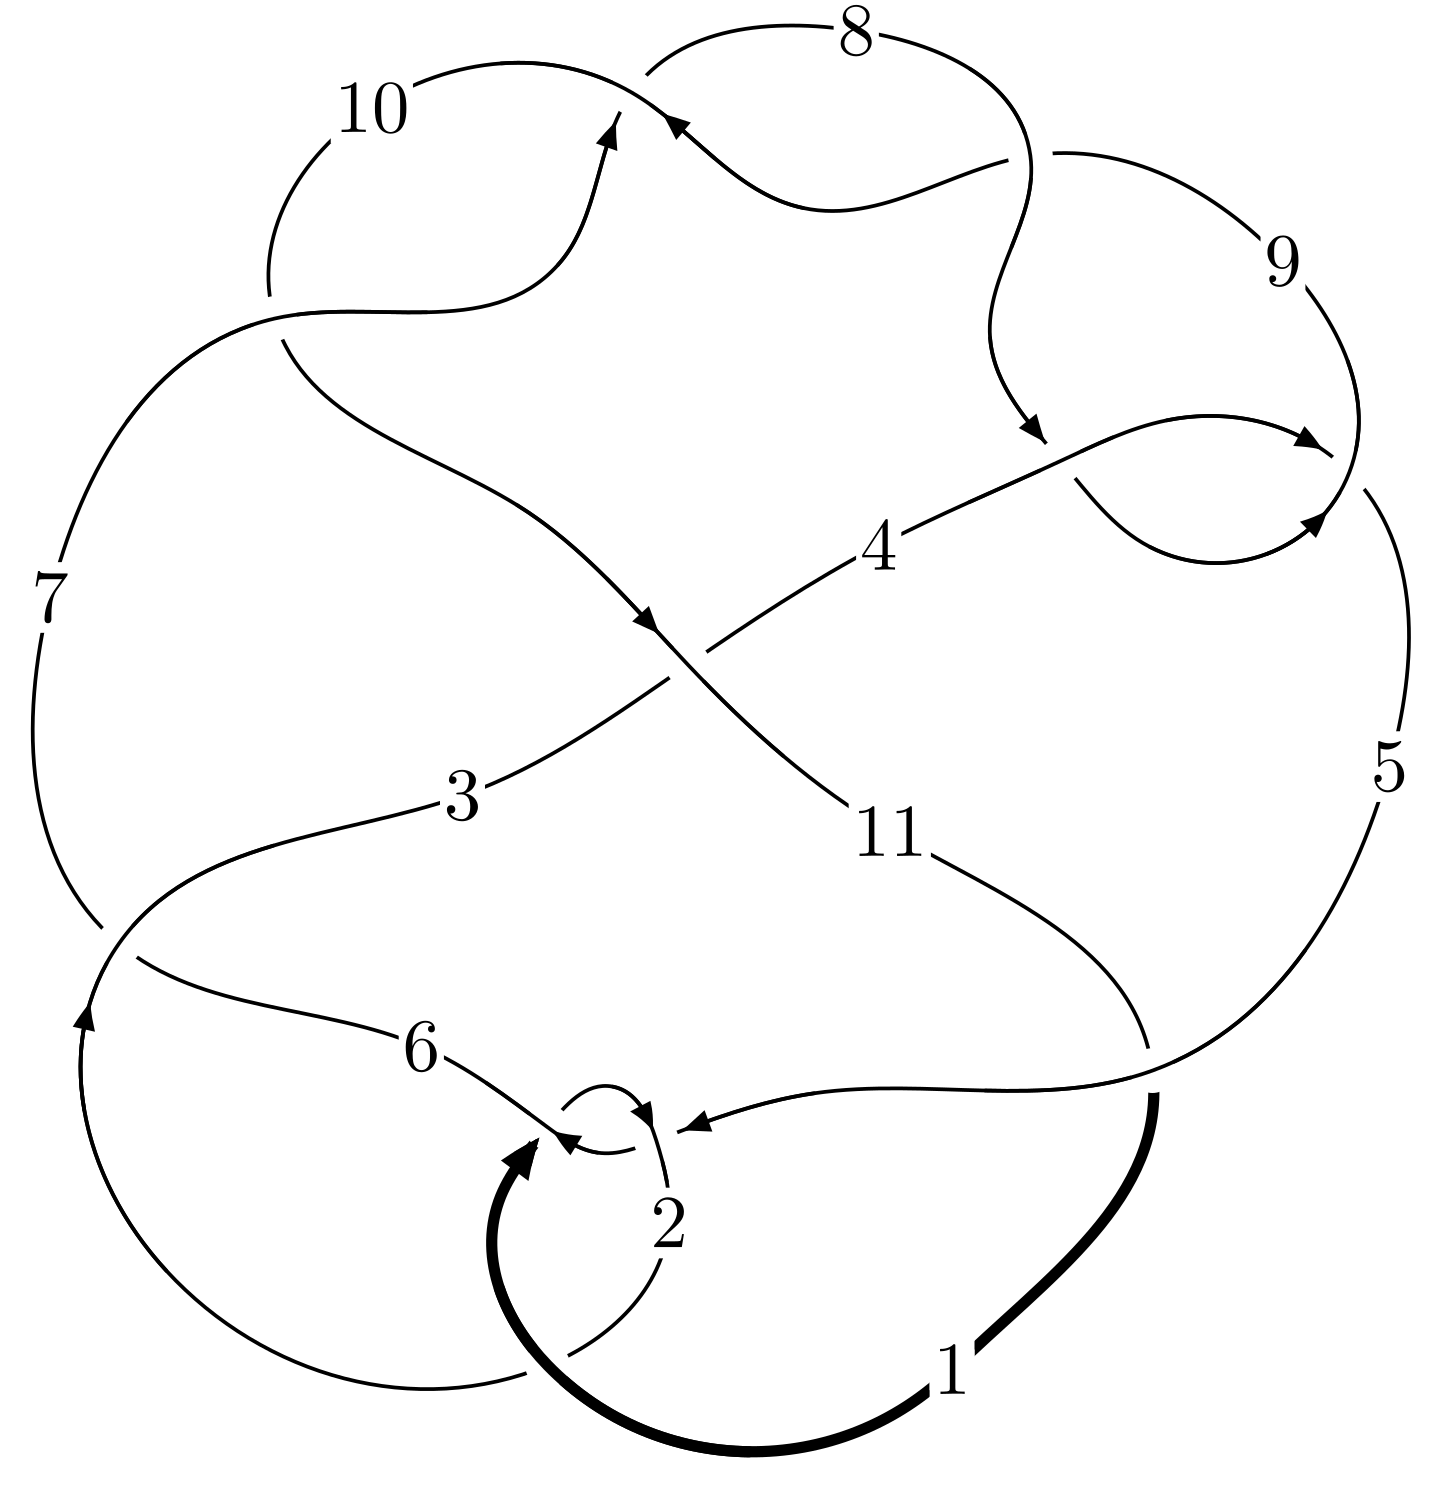
\includegraphics[width=112pt]{../../../GIT/diagram.site/Diagrams/png/342_11a_93.png}\\
\ \ \ A knot diagram\footnotemark}&
\allowdisplaybreaks
\textbf{Linearized knot diagam} \\
\cline{2-2}
 &
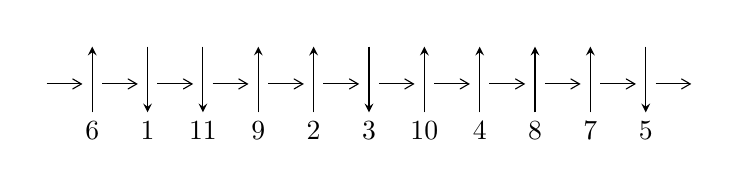
\begin{tikzpicture}[x=20pt, y=17pt]
	% nodes
	\node (C0) at (0, 0) {};
	\node (C1) at (1, 0) {};
	\node (C1U) at (1, +1) {};
	\node (C1D) at (1, -1) {6};

	\node (C2) at (2, 0) {};
	\node (C2U) at (2, +1) {};
	\node (C2D) at (2, -1) {1};

	\node (C3) at (3, 0) {};
	\node (C3U) at (3, +1) {};
	\node (C3D) at (3, -1) {11};

	\node (C4) at (4, 0) {};
	\node (C4U) at (4, +1) {};
	\node (C4D) at (4, -1) {9};

	\node (C5) at (5, 0) {};
	\node (C5U) at (5, +1) {};
	\node (C5D) at (5, -1) {2};

	\node (C6) at (6, 0) {};
	\node (C6U) at (6, +1) {};
	\node (C6D) at (6, -1) {3};

	\node (C7) at (7, 0) {};
	\node (C7U) at (7, +1) {};
	\node (C7D) at (7, -1) {10};

	\node (C8) at (8, 0) {};
	\node (C8U) at (8, +1) {};
	\node (C8D) at (8, -1) {4};

	\node (C9) at (9, 0) {};
	\node (C9U) at (9, +1) {};
	\node (C9D) at (9, -1) {8};

	\node (C10) at (10, 0) {};
	\node (C10U) at (10, +1) {};
	\node (C10D) at (10, -1) {7};

	\node (C11) at (11, 0) {};
	\node (C11U) at (11, +1) {};
	\node (C11D) at (11, -1) {5};
	\node (C12) at (12, 0) {};

	% arrows
	\draw[->,>={angle 60}]
	(C0) edge (C1) (C1) edge (C2) (C2) edge (C3) (C3) edge (C4) (C4) edge (C5) (C5) edge (C6) (C6) edge (C7) (C7) edge (C8) (C8) edge (C9) (C9) edge (C10) (C10) edge (C11) (C11) edge (C12) ;	\draw[->,>=stealth]
	(C1D) edge (C1U) (C2U) edge (C2D) (C3U) edge (C3D) (C4D) edge (C4U) (C5D) edge (C5U) (C6U) edge (C6D) (C7D) edge (C7U) (C8D) edge (C8U) (C9D) edge (C9U) (C10D) edge (C10U) (C11U) edge (C11D) ;
	\end{tikzpicture} \\
\hhline{~~} \\& 
\textbf{Solving Sequence} \\ \cline{2-2} 
 &
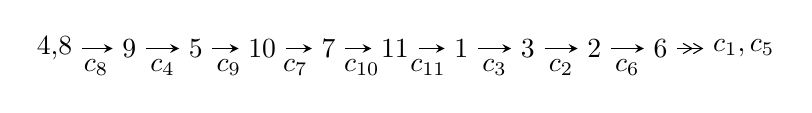
\begin{tikzpicture}[x=24pt, y=7pt]
	% node
	\node (A0) at (-1/8, 0) {4,8};
	\node (A1) at (1, 0) {9};
	\node (A2) at (2, 0) {5};
	\node (A3) at (3, 0) {10};
	\node (A4) at (4, 0) {7};
	\node (A5) at (5, 0) {11};
	\node (A6) at (6, 0) {1};
	\node (A7) at (7, 0) {3};
	\node (A8) at (8, 0) {2};
	\node (A9) at (9, 0) {6};
	\node (C1) at (1/2, -1) {$c_{8}$};
	\node (C2) at (3/2, -1) {$c_{4}$};
	\node (C3) at (5/2, -1) {$c_{9}$};
	\node (C4) at (7/2, -1) {$c_{7}$};
	\node (C5) at (9/2, -1) {$c_{10}$};
	\node (C6) at (11/2, -1) {$c_{11}$};
	\node (C7) at (13/2, -1) {$c_{3}$};
	\node (C8) at (15/2, -1) {$c_{2}$};
	\node (C9) at (17/2, -1) {$c_{6}$};
	\node (A10) at (41/4, 0) {$c_{1},c_{5}$};

	% edge
	\draw[->,>=stealth]	
	(A0) edge (A1) (A1) edge (A2) (A2) edge (A3) (A3) edge (A4) (A4) edge (A5) (A5) edge (A6) (A6) edge (A7) (A7) edge (A8) (A8) edge (A9) ;
	\draw[->>,>={angle 60}]	
	(A9) edge (A10);
\end{tikzpicture} \\ 

\end{tabular} \\

\footnotetext{
The image of knot diagram is generated by the software ``\textbf{Draw programme}" developed by Andrew Bartholomew(\url{http://www.layer8.co.uk/maths/draw/index.htm\#Running-draw}), where we modified some parts for our purpose(\url{https://github.com/CATsTAILs/LinksPainter}).
}\phantom \\ \newline 
\centering \textbf{Ideals for irreducible components\footnotemark of $X_{\text{par}}$} 
 
\begin{align*}
I^u_{1}&=\langle 
u^{46}- u^{45}+\cdots- u+1\rangle \\
\\
\end{align*}
\raggedright * 1 irreducible components of $\dim_{\mathbb{C}}=0$, with total 46 representations.\\
\footnotetext{All coefficients of polynomials are rational numbers. But the coefficients are sometimes approximated in decimal forms when there is not enough margin.}
\newpage
\renewcommand{\arraystretch}{1}
\centering \section*{I. $I^u_{1}= \langle u^{46}- u^{45}+\cdots- u+1 \rangle$}
\flushleft \textbf{(i) Arc colorings}\\
\begin{tabular}{m{7pt} m{180pt} m{7pt} m{180pt} }
\flushright $a_{4}=$&$\begin{pmatrix}0\\u\end{pmatrix}$ \\
\flushright $a_{8}=$&$\begin{pmatrix}1\\0\end{pmatrix}$ \\
\flushright $a_{9}=$&$\begin{pmatrix}1\\- u^2\end{pmatrix}$ \\
\flushright $a_{5}=$&$\begin{pmatrix}u\\- u^3+u\end{pmatrix}$ \\
\flushright $a_{10}=$&$\begin{pmatrix}- u^2+1\\- u^2\end{pmatrix}$ \\
\flushright $a_{7}=$&$\begin{pmatrix}u^4- u^2+1\\u^4\end{pmatrix}$ \\
\flushright $a_{11}=$&$\begin{pmatrix}- u^6+u^4-2 u^2+1\\- u^6- u^2\end{pmatrix}$ \\
\flushright $a_{1}=$&$\begin{pmatrix}u^{10}- u^8+2 u^6- u^4- u^2+1\\- u^{12}+2 u^{10}-4 u^8+4 u^6-3 u^4\end{pmatrix}$ \\
\flushright $a_{3}=$&$\begin{pmatrix}u^{13}-2 u^{11}+5 u^9-6 u^7+6 u^5-4 u^3+u\\u^{13}- u^{11}+3 u^9-2 u^7+2 u^5- u^3+u\end{pmatrix}$ \\
\flushright $a_{2}=$&$\begin{pmatrix}u^{35}-4 u^{33}+\cdots-7 u^3+2 u\\- u^{37}+5 u^{35}+\cdots- u^3+u\end{pmatrix}$ \\
\flushright $a_{6}=$&$\begin{pmatrix}- u^{22}+3 u^{20}+\cdots-2 u^2+1\\- u^{22}+2 u^{20}+\cdots+4 u^4- u^2\end{pmatrix}$\\ \flushright $a_{6}=$&$\begin{pmatrix}- u^{22}+3 u^{20}+\cdots-2 u^2+1\\- u^{22}+2 u^{20}+\cdots+4 u^4- u^2\end{pmatrix}$\\&\end{tabular}
\flushleft \textbf{(ii) Obstruction class $= -1$}\\~\\
\flushleft \textbf{(iii) Cusp Shapes $= -4 u^{44}+4 u^{43}+\cdots-4 u+2$}\\~\\
\newpage\renewcommand{\arraystretch}{1}
\flushleft \textbf{(iv) u-Polynomials at the component}\newline \\
\begin{tabular}{m{50pt}|m{274pt}}
Crossings & \hspace{64pt}u-Polynomials at each crossing \\
\hline $$\begin{aligned}c_{1},c_{5}\end{aligned}$$&$\begin{aligned}
&u^{46}- u^{45}+\cdots-3 u+1
\end{aligned}$\\
\hline $$\begin{aligned}c_{2}\end{aligned}$$&$\begin{aligned}
&u^{46}+25 u^{45}+\cdots- u+1
\end{aligned}$\\
\hline $$\begin{aligned}c_{3}\end{aligned}$$&$\begin{aligned}
&u^{46}-7 u^{45}+\cdots+25 u+101
\end{aligned}$\\
\hline $$\begin{aligned}c_{4},c_{8}\end{aligned}$$&$\begin{aligned}
&u^{46}+u^{45}+\cdots+u+1
\end{aligned}$\\
\hline $$\begin{aligned}c_{6},c_{11}\end{aligned}$$&$\begin{aligned}
&u^{46}+u^{45}+\cdots+11 u+2
\end{aligned}$\\
\hline $$\begin{aligned}c_{7},c_{9},c_{10}\end{aligned}$$&$\begin{aligned}
&u^{46}-11 u^{45}+\cdots- u+1
\end{aligned}$\\
\hline
\end{tabular}\\~\\
\newpage\renewcommand{\arraystretch}{1}
\flushleft \textbf{(v) Riley Polynomials at the component}\newline \\
\begin{tabular}{m{50pt}|m{274pt}}
Crossings & \hspace{64pt}Riley Polynomials at each crossing \\
\hline $$\begin{aligned}c_{1},c_{5}\end{aligned}$$&$\begin{aligned}
&y^{46}+25 y^{45}+\cdots- y+1
\end{aligned}$\\
\hline $$\begin{aligned}c_{2}\end{aligned}$$&$\begin{aligned}
&y^{46}-7 y^{45}+\cdots-17 y+1
\end{aligned}$\\
\hline $$\begin{aligned}c_{3}\end{aligned}$$&$\begin{aligned}
&y^{46}-19 y^{45}+\cdots+139967 y+10201
\end{aligned}$\\
\hline $$\begin{aligned}c_{4},c_{8}\end{aligned}$$&$\begin{aligned}
&y^{46}-11 y^{45}+\cdots- y+1
\end{aligned}$\\
\hline $$\begin{aligned}c_{6},c_{11}\end{aligned}$$&$\begin{aligned}
&y^{46}-39 y^{45}+\cdots+239 y+4
\end{aligned}$\\
\hline $$\begin{aligned}c_{7},c_{9},c_{10}\end{aligned}$$&$\begin{aligned}
&y^{46}+49 y^{45}+\cdots-9 y+1
\end{aligned}$\\
\hline
\end{tabular}\\~\\
\newpage\flushleft \textbf{(vi) Complex Volumes and Cusp Shapes}
$$\begin{array}{c|c|c}  
\text{Solutions to }I^u_{1}& \I (\text{vol} + \sqrt{-1}CS) & \text{Cusp shape}\\
 \hline 
\begin{aligned}
u &= \phantom{-}0.926616 + 0.410566 I\end{aligned}
 & -0.61712 + 4.64033 I & \phantom{-}3.90866 - 6.37467 I \\ \hline\begin{aligned}
u &= \phantom{-}0.926616 - 0.410566 I\end{aligned}
 & -0.61712 - 4.64033 I & \phantom{-}3.90866 + 6.37467 I \\ \hline\begin{aligned}
u &= -0.914147 + 0.454246 I\end{aligned}
 & -4.39692 - 0.74190 I & -1.01050 + 2.76153 I \\ \hline\begin{aligned}
u &= -0.914147 - 0.454246 I\end{aligned}
 & -4.39692 + 0.74190 I & -1.01050 - 2.76153 I \\ \hline\begin{aligned}
u &= \phantom{-}0.911781 + 0.304147 I\end{aligned}
 & \phantom{-}2.15395 + 4.51135 I & \phantom{-}7.09548 - 8.74151 I \\ \hline\begin{aligned}
u &= \phantom{-}0.911781 - 0.304147 I\end{aligned}
 & \phantom{-}2.15395 - 4.51135 I & \phantom{-}7.09548 + 8.74151 I \\ \hline\begin{aligned}
u &= -0.954952 + 0.418436 I\end{aligned}
 & -3.69312 - 9.28862 I & \phantom{-}0.73867 + 9.25644 I \\ \hline\begin{aligned}
u &= -0.954952 - 0.418436 I\end{aligned}
 & -3.69312 + 9.28862 I & \phantom{-}0.73867 - 9.25644 I \\ \hline\begin{aligned}
u &= \phantom{-}0.930509 + 0.048833 I\end{aligned}
 & -1.66163 - 4.02262 I & \phantom{-}4.31758 + 3.30145 I \\ \hline\begin{aligned}
u &= \phantom{-}0.930509 - 0.048833 I\end{aligned}
 & -1.66163 + 4.02262 I & \phantom{-}4.31758 - 3.30145 I \\ \hline\begin{aligned}
u &= -0.890449 + 0.239219 I\end{aligned}
 & \phantom{-}2.52825 - 0.40745 I & \phantom{-}9.12909 + 0.87770 I \\ \hline\begin{aligned}
u &= -0.890449 - 0.239219 I\end{aligned}
 & \phantom{-}2.52825 + 0.40745 I & \phantom{-}9.12909 - 0.87770 I \\ \hline\begin{aligned}
u &= -0.814350 + 0.077554 I\end{aligned}
 & \phantom{-}1.220450 - 0.051921 I & \phantom{-}8.69452 + 0.37904 I \\ \hline\begin{aligned}
u &= -0.814350 - 0.077554 I\end{aligned}
 & \phantom{-}1.220450 + 0.051921 I & \phantom{-}8.69452 - 0.37904 I \\ \hline\begin{aligned}
u &= -0.845736 + 0.830186 I\end{aligned}
 & -4.84996 + 2.01035 I & \phantom{-0.000000 } 0. - 3.31970 I \\ \hline\begin{aligned}
u &= -0.845736 - 0.830186 I\end{aligned}
 & -4.84996 - 2.01035 I & \phantom{-0.000000 -}0. + 3.31970 I \\ \hline\begin{aligned}
u &= \phantom{-}0.871966 + 0.808985 I\end{aligned}
 & -3.65550 + 2.31659 I & \phantom{-}2.70777 - 2.80879 I \\ \hline\begin{aligned}
u &= \phantom{-}0.871966 - 0.808985 I\end{aligned}
 & -3.65550 - 2.31659 I & \phantom{-}2.70777 + 2.80879 I \\ \hline\begin{aligned}
u &= \phantom{-}0.918456 + 0.798302 I\end{aligned}
 & -3.51223 + 3.71082 I & \phantom{-}3.02524 - 2.42011 I \\ \hline\begin{aligned}
u &= \phantom{-}0.918456 - 0.798302 I\end{aligned}
 & -3.51223 - 3.71082 I & \phantom{-}3.02524 + 2.42011 I \\ \hline\begin{aligned}
u &= -0.851134 + 0.882685 I\end{aligned}
 & -8.86024 + 1.86315 I &                  -6
-1.106545 + 0. 10   I\phantom{ +0.000000I} \\ \hline\begin{aligned}
u &= -0.851134 - 0.882685 I\end{aligned}
 & -8.86024 - 1.86315 I &                  -6
-1.106545 + 0. 10   I\phantom{ +0.000000I} \\ \hline\begin{aligned}
u &= \phantom{-}0.845372 + 0.890503 I\end{aligned}
 & -12.13790 - 6.72244 I & -4.11786 + 3.49282 I \\ \hline\begin{aligned}
u &= \phantom{-}0.845372 - 0.890503 I\end{aligned}
 & -12.13790 + 6.72244 I & -4.11786 - 3.49282 I \\ \hline\begin{aligned}
u &= \phantom{-}0.862272 + 0.887980 I\end{aligned}
 & -12.90310 + 2.35522 I & -5.23797 - 2.80998 I \\ \hline\begin{aligned}
u &= \phantom{-}0.862272 - 0.887980 I\end{aligned}
 & -12.90310 - 2.35522 I & -5.23797 + 2.80998 I \\ \hline\begin{aligned}
u &= -0.943172 + 0.803061 I\end{aligned}
 & -4.55090 - 8.11388 I & \phantom{-0.000000 -}0. + 8.45293 I \\ \hline\begin{aligned}
u &= -0.943172 - 0.803061 I\end{aligned}
 & -4.55090 + 8.11388 I & \phantom{-0.000000 } 0. - 8.45293 I \\ \hline\begin{aligned}
u &= \phantom{-}0.640742 + 0.410350 I\end{aligned}
 & -1.44816 + 1.63407 I & -3.46961 - 5.26360 I \\ \hline\begin{aligned}
u &= \phantom{-}0.640742 - 0.410350 I\end{aligned}
 & -1.44816 - 1.63407 I & -3.46961 + 5.26360 I\\
 \hline 
 \end{array}$$\newpage$$\begin{array}{c|c|c}  
\text{Solutions to }I^u_{1}& \I (\text{vol} + \sqrt{-1}CS) & \text{Cusp shape}\\
 \hline 
\begin{aligned}
u &= -0.907049 + 0.844230 I\end{aligned}
 & -8.35989 - 3.13875 I & -5.65909 + 2.64059 I \\ \hline\begin{aligned}
u &= -0.907049 - 0.844230 I\end{aligned}
 & -8.35989 + 3.13875 I & -5.65909 - 2.64059 I \\ \hline\begin{aligned}
u &= -0.391409 + 0.635070 I\end{aligned}
 & -6.04130 - 3.27213 I & -5.13047 + 3.47488 I \\ \hline\begin{aligned}
u &= -0.391409 - 0.635070 I\end{aligned}
 & -6.04130 + 3.27213 I & -5.13047 - 3.47488 I \\ \hline\begin{aligned}
u &= -0.966860 + 0.834394 I\end{aligned}
 & -8.49402 - 8.22551 I & \phantom{-0.000000 -}0. + 5.24210 I \\ \hline\begin{aligned}
u &= -0.966860 - 0.834394 I\end{aligned}
 & -8.49402 + 8.22551 I & \phantom{-0.000000 } 0. - 5.24210 I \\ \hline\begin{aligned}
u &= \phantom{-}0.963540 + 0.844204 I\end{aligned}
 & -12.58150 + 4.05580 I & -4.67518 + 0. I\phantom{ +0.000000I} \\ \hline\begin{aligned}
u &= \phantom{-}0.963540 - 0.844204 I\end{aligned}
 & -12.58150 - 4.05580 I & -4.67518 + 0. I\phantom{ +0.000000I} \\ \hline\begin{aligned}
u &= -0.313493 + 0.645402 I\end{aligned}
 & -5.71816 + 5.39161 I & -4.52962 - 3.70458 I \\ \hline\begin{aligned}
u &= -0.313493 - 0.645402 I\end{aligned}
 & -5.71816 - 5.39161 I & -4.52962 + 3.70458 I \\ \hline\begin{aligned}
u &= \phantom{-}0.974549 + 0.835372 I\end{aligned}
 & -11.7284 + 13.1112 I & \phantom{-0.000000 } 0. - 8.32350 I \\ \hline\begin{aligned}
u &= \phantom{-}0.974549 - 0.835372 I\end{aligned}
 & -11.7284 - 13.1112 I & \phantom{-0.000000 -}0. + 8.32350 I \\ \hline\begin{aligned}
u &= \phantom{-}0.339399 + 0.599164 I\end{aligned}
 & -2.45150 - 0.89325 I & -1.50590 + 0.29908 I \\ \hline\begin{aligned}
u &= \phantom{-}0.339399 - 0.599164 I\end{aligned}
 & -2.45150 + 0.89325 I & -1.50590 - 0.29908 I \\ \hline\begin{aligned}
u &= \phantom{-}0.107548 + 0.462569 I\end{aligned}
 & -0.09670 - 1.71368 I & -0.09766 + 4.16841 I \\ \hline\begin{aligned}
u &= \phantom{-}0.107548 - 0.462569 I\end{aligned}
 & -0.09670 + 1.71368 I & -0.09766 - 4.16841 I\\
 \hline 
 \end{array}$$\newpage
\newpage\renewcommand{\arraystretch}{1}
\centering \section*{ II. u-Polynomials}
\begin{tabular}{m{50pt}|m{274pt}}
Crossings & \hspace{64pt}u-Polynomials at each crossing \\
\hline $$\begin{aligned}c_{1},c_{5}\end{aligned}$$&$\begin{aligned}
&u^{46}- u^{45}+\cdots-3 u+1
\end{aligned}$\\
\hline $$\begin{aligned}c_{2}\end{aligned}$$&$\begin{aligned}
&u^{46}+25 u^{45}+\cdots- u+1
\end{aligned}$\\
\hline $$\begin{aligned}c_{3}\end{aligned}$$&$\begin{aligned}
&u^{46}-7 u^{45}+\cdots+25 u+101
\end{aligned}$\\
\hline $$\begin{aligned}c_{4},c_{8}\end{aligned}$$&$\begin{aligned}
&u^{46}+u^{45}+\cdots+u+1
\end{aligned}$\\
\hline $$\begin{aligned}c_{6},c_{11}\end{aligned}$$&$\begin{aligned}
&u^{46}+u^{45}+\cdots+11 u+2
\end{aligned}$\\
\hline $$\begin{aligned}c_{7},c_{9},c_{10}\end{aligned}$$&$\begin{aligned}
&u^{46}-11 u^{45}+\cdots- u+1
\end{aligned}$\\
\hline
\end{tabular}\newpage\renewcommand{\arraystretch}{1}
\centering \section*{ III. Riley Polynomials}
\begin{tabular}{m{50pt}|m{274pt}}
Crossings & \hspace{64pt}Riley Polynomials at each crossing \\
\hline $$\begin{aligned}c_{1},c_{5}\end{aligned}$$&$\begin{aligned}
&y^{46}+25 y^{45}+\cdots- y+1
\end{aligned}$\\
\hline $$\begin{aligned}c_{2}\end{aligned}$$&$\begin{aligned}
&y^{46}-7 y^{45}+\cdots-17 y+1
\end{aligned}$\\
\hline $$\begin{aligned}c_{3}\end{aligned}$$&$\begin{aligned}
&y^{46}-19 y^{45}+\cdots+139967 y+10201
\end{aligned}$\\
\hline $$\begin{aligned}c_{4},c_{8}\end{aligned}$$&$\begin{aligned}
&y^{46}-11 y^{45}+\cdots- y+1
\end{aligned}$\\
\hline $$\begin{aligned}c_{6},c_{11}\end{aligned}$$&$\begin{aligned}
&y^{46}-39 y^{45}+\cdots+239 y+4
\end{aligned}$\\
\hline $$\begin{aligned}c_{7},c_{9},c_{10}\end{aligned}$$&$\begin{aligned}
&y^{46}+49 y^{45}+\cdots-9 y+1
\end{aligned}$\\
\hline
\end{tabular}
\vskip 2pc
\end{document}